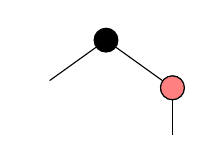
\begin{tikzpicture}[transform shape, scale=0.8, baseline=(current bounding box.center)]
	\begin{scope}[nodes={draw=black, circle, minimum width=2.5ex}, sibling distance=6em, level distance=5ex]
		\draw node (root) [fill=black] {}
		child {node [draw=none] {}}
		child {
				node [fill=red!50] {}
				child node [draw=none] {}
				child node [fill=red!50] {}
			}
		;
	\end{scope}
\end{tikzpicture}
\begin{tikzpicture}
	\draw node [minimum width=3em] {\( \Longrightarrow \)};
\end{tikzpicture}
\begin{tikzpicture}[transform shape, scale=0.8, baseline=(current bounding box.center)]\begin{scope}[nodes={draw=black, circle, minimum width=2.5ex}, sibling distance=6em, level distance=5ex]
		\draw node (root) [fill=black] {}
		child [child anchor=apex] {
				node [isosceles triangle, shape border rotate=90, anchor=apex, minimum width=2em] {}
			}
		child {
				node (ellipsis) [draw=none] {\( \ddots \)}
				child { node [draw=none] {} edge from parent [draw=none] }
				child {
						node (replacing) [fill=black] {}
						child [child anchor=apex, sibling distance=3.5em] {
								node (left) [isosceles triangle, shape border rotate=90, anchor=apex, minimum width=2em] {}
							}
						child [child anchor=apex, sibling distance=3.5em] {
								node (rightmost) [isosceles triangle, shape border rotate=90, anchor=apex, minimum width=2em] {}
							}
					}
			}
		;
	\end{scope}
	% * NOTE ellipsis.340 => apenas para a chave ficar mais paralela
	\draw [decorate, decoration={brace, amplitude=7pt, raise=1em}] (root.north) -- (ellipsis.340) node [pos=0.5, above right=2em] {\( x \) nós pretos};
	\draw [decorate, decoration={brace, amplitude=7pt, raise=1.5em}]  (replacing.north -| rightmost.south) -- (rightmost.south) node [pos=0.5, right=3em] {\( y \) nós pretos};
	\draw [dashed, draw=black!50] ($(replacing.north) + (90:1em)$) -- ($(left.left corner) + (205:1em)$) -- ($(rightmost.right corner) + (335:1em)$) -- cycle;
\end{tikzpicture}